The science payload includes a mid-band phased array operating from 300--900 MHz, a wide band and high band antenna (600-1800 MHz), an ``FM'' band antenna (60--110 MHz), and a low band antenna (1--50 MHz). A schematic of the payload is shown in Figure \ref{fig:block}.

\begin{figure}
	\centering
	\includegraphics[width=\linewidth]{figures/blockdiagram.png}
	\caption{Block diagram of the science payload.\label{fig:block}}
\end{figure}

The mid-band array covers the bulk of the lander top surface with 48 dual polarizatio wideband antenna elements. The array forms a fan of beams on the sky designed to cover most of the lunar sky over time (Fig.\ \ref{fig:midband_beam_maps}). Formed beam output signals are downconverted and sampled in a 50 MHz subband that is tuned scanned repeatedly across the array operating bandwidth. 

\begin{figure}
	\centering
	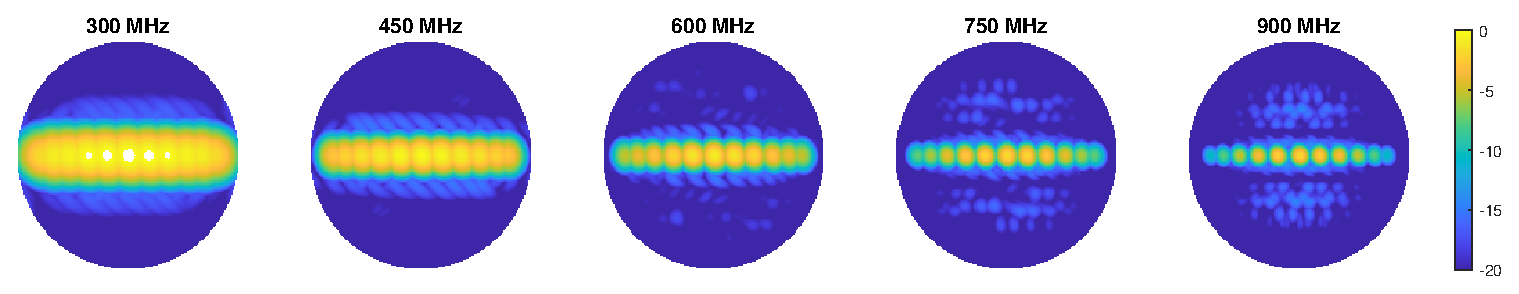
\includegraphics[width=\linewidth]{figures/midband_array_28cm_3dBSLL_beams_max.eps}
	\caption{Midband array formed beams over frequency. Scale is aperture efficiency in dB relative to a 3 meter diameter area. Beams are centered within 11 equal intervals over a 120 degree field of view.}
	\label{fig:midband_beam_maps}
\end{figure}

\begin{figure}
	\centering
	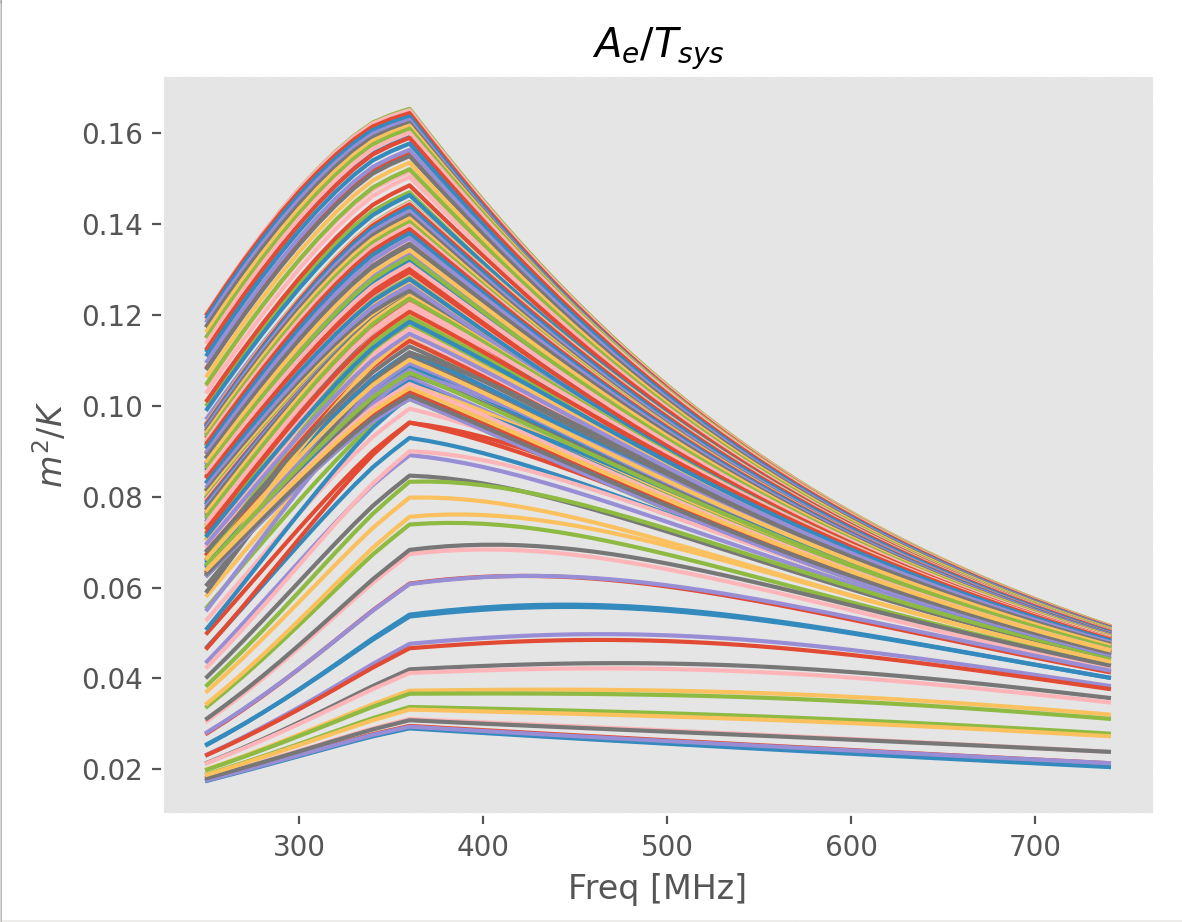
\includegraphics[width=0.5\linewidth]{figures/sensitivity_early_est.png}
	\caption{Early estimates of sensitivity showing the range of the sensitivity for different portions of the Galaxy.\label{sensitivity}}
\end{figure}

\begin{figure}
	\centering
	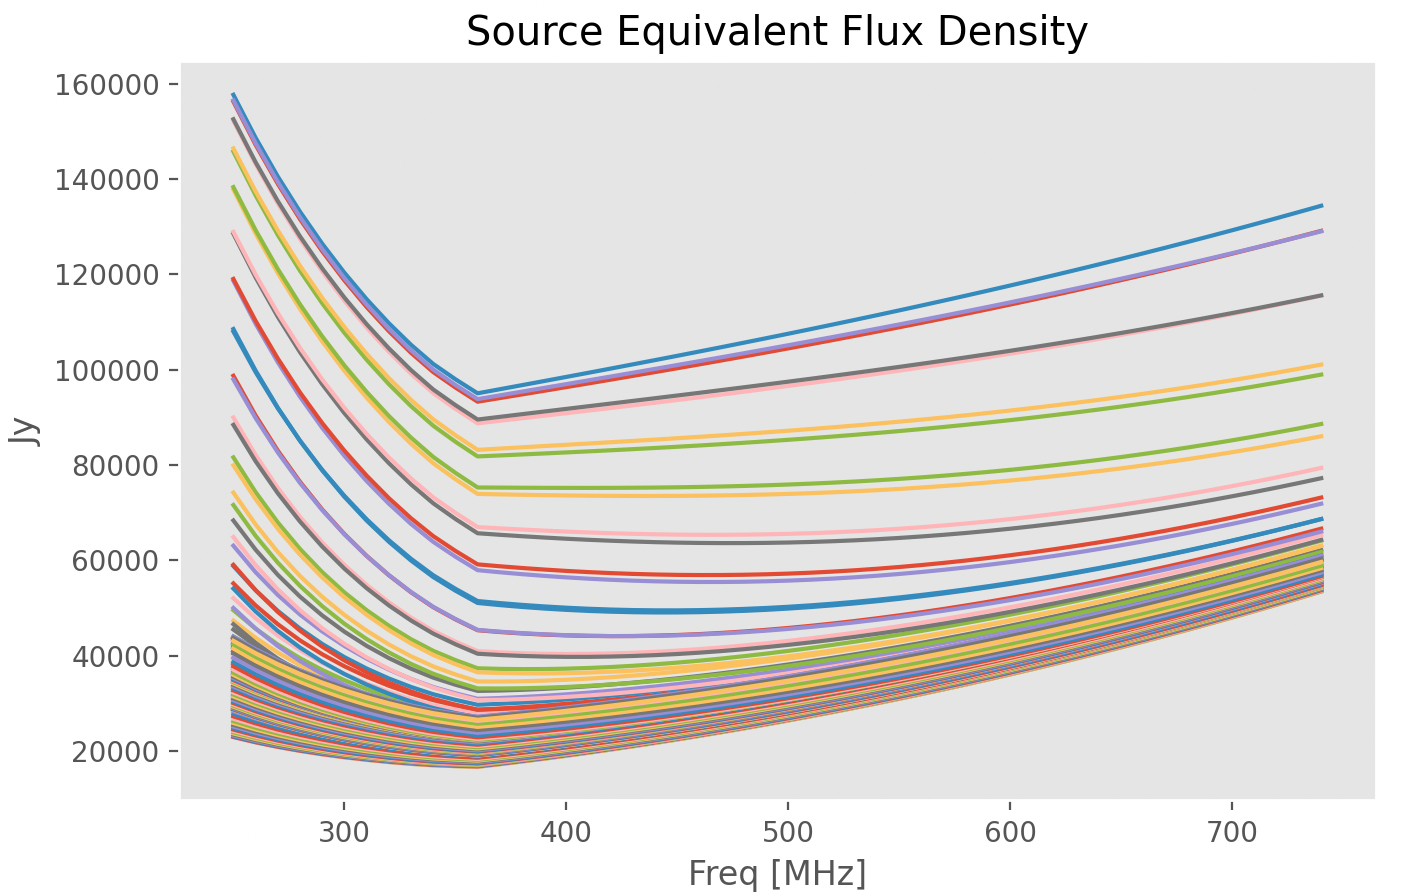
\includegraphics[width=0.75\linewidth]{figures/sefd.png}
	\caption{Early estimates of sensitivity showing the range of the sensitivity for different portions of the Galaxy in source equivalent flux density.\label{sefd}}
\end{figure}